\documentclass[9pt,twocolumn,twoside,lineno]{pnas-new}
% Use the lineno option to display guide line numbers if required.

\templatetype{pnasresearcharticle} % Choose template 
% {pnasresearcharticle} = Template for a two-column research article
% {pnasmathematics} %= Template for a one-column mathematics article
% {pnasinvited} %= Template for a PNAS invited submission

\title{Does reducing malaria's burden cause economic growth, or does growth reduce malaria?}

% Use letters for affiliations, numbers to show equal authorship (if applicable) and to indicate the corresponding author
\author[a,b,1]{Joe Brew}
\author[a]{Laia Cirera} 
\author[a,c]{Elisa Sicuri}

\affil[a]{Barcelona Institute for Global Health: c/ Rosselló, 132, 5è 2a. 08036, Barcelona, Catalonia}
\affil[b]{VU University Amsterdam: De Boelelaan 1105, 1081 HV Amsterdam, Netherlands}
\affil[c]{Imperial College London: South Kensington Campus, London SW7 2AZ, U.K., UK}

% Please give the surname of the lead author for the running footer
\leadauthor{Brew} 

% Please add here a significance statement to explain the relevance of your work
\significancestatement{Though it is clear that malaria is a "disease of poverty", the extent to which malaria is the cause or effect of poverty is not fully understood. Identifying the direction of the causal relationship between health and wealth is vital to knowing where resources should be directed, ie whether interventions in poor, malaria-endemic societies should target the disease or the poverty. We analyzed the relationship between GDP growth and the prevalence of Plasmodium falciparum among children in 27 malaria-endemic African countries, and identified health to wealth as the primary causal pathway. Our findings suggest that scaling up investment in reducing malaria's burden could be a pre-requisite condition for enabling economic growth in Sub-Saharan Africa.}

% Please include corresponding author, author contribution and author declaration information
\authorcontributions{Author contributions: J.B., L.C., and E.S. designed research; J.B. gathered and processed data; J.B., L.C., and E.S. analyzed
data; J.B., L.C., and E.S. wrote the paper}
\authordeclaration{The authors declare no conflicts of interest}
\correspondingauthor{\textsuperscript{1}E-mail: joebrew@gmail.com}

% Keywords are not mandatory, but authors are strongly encouraged to provide them. If provided, please include two to five keywords, separated by the pipe symbol, e.g:
\keywords{Malaria $|$ Economics $|$ Development $|$ Growth $|$ Causality} 

\begin{abstract}
The correlation between poverty and malaria endemicity has been well established, but causal directionality has not. Understanding the extent to which malaria causes economic stagnation, and vice-versa, is important for an efficient allotment of development resources. Using 15 years of panel data from 27 malaria-endemic Sub-Saharan African countries, we carry out a Granger-causality analysis of the potential directional relationship between economic growth and a reduction in malaria’s prevalence. Having identified a temporally coherent health-to-wealth pathway, we then carry out a sensitivity analysis to test causality. Our results are robust, suggesting that development-oriented aid and investment in malaria-endemic countries should prioritize those interventions which reduce malaria directly.
\end{abstract}

\dates{This manuscript was compiled on \today}
\doi{\url{www.pnas.org/cgi/doi/10.1073/pnas.XXXXXXXXXX}}

\begin{document}

\maketitle
\thispagestyle{firststyle}
\ifthenelse{\boolean{shortarticle}}{\ifthenelse{\boolean{singlecolumn}}{\abscontentformatted}{\abscontent}}{}


\dropcap{M}alaria causes more than a half million deaths worldwide every year \cite{White}. In addition to its devastating health effects, Malaria has a large economic impact.  By reducing one’s ability to work efficiently \cite{Nonvignon2016-vt}, if at all, malaria imposes a large financial cost on the infected \cite{Asenso-Okyere1997-wj} \cite{Ajani2010-dd}, and the toll trickles upwards to society at large \cite{Sachs2002-ig}. Not only does malaria likely has a negative effect on GDP and growth \cite{McCarthy2000-wl, Orem2012-kr, Hong2011-sa, Sachs2002-ig}, in a classic feedback loop, low growth can keep societies in a resource-scarce state making interventions which target the control or elimination of malaria difficult \cite{White, Purdy2013-rt, Howard2017-pk, Phillips1998-ky}. 

The correlation between poverty and malaria endemicity has been well established, but causal directionality has not. This lack of clarity may partially explain why there are two schools of thought in development circles regarding where resources should be directed. One school argues that a society must be brought out of poverty, after which gains in health are almost inevitable, but prior to which significant health improvements are nearly impossible \cite{Musgrove1996-hm}.  The other argues for a more “holistic” development approach, implicitly calling for resources to be devoted to areas believed to be pre-requiste to wealth acquisition, such as health \cite{Storm2008-dd, Sen_undated-gp}.  Clarke et al. covers this distinction more thoroughly \cite{Clarke_JA2016-ik}.

Though both schools acknowledge that the interaction between health and wealth is bi-directional, understanding the extent to which malaria’s burden affects the economy, and vice-versa, could shed light on areas where developmentalists should focus in order to break the vicious cycle. Particularly, knowing which kinds of improvements precede the other helps to guide policies which aim to improve well-being in the long-term. Since malaria’s economic effects are at the macro-scale, a randomized controlled trial to assess the extent to which a controlled shock to the burden of malaria or the economy is not feasible. Ample experiments and interventions exist at the sub-national level, and occasionally the national level, but these are generally carried out in isolation, lacking the plausible counterfactual with which to compare any observed improvement in malaria’s burden or economic growth. Additionally, at the sub-national and national levels, the amount of confounding factors (political changes, climate crises, etc.) are too great to isolate causal effects. 

Given the impossibility of parsing these many complex factors at the micro-level, one approach for understanding causal directionality in the malaria-economy relationship is to zoom out to the macro-level and focus on simple temporality (ie, whether changes to the economy tend to preceed changes to malaria’s burden or vice-versa). By including many countries rather than just one, we cancel out each one’s idiosyncracies, and by carrying out statistical precedence analysis, we can identify a potentially causal trend for further analysis. 

Granger-causation analysis, a form of temporal precedence analysis, is a useful tool for doing this \cite{Granger_undated-wn, Molenaar2018-ss, Koller2016-rv, Granger1896-di, Clarke_JA2016-ik}. In the field of Economics, it is commonly used with panel data to assess the directionality of a bi-directional relationship \cite{Law_2013, Joerding1986}. For ths specific link to health and growth, it has been used to examine the causal links between the health status and savings of elderly Europeans \cite{Andreyeva2007-zq}, general health and socieconomic status \cite{Adams2003-wl}, and macro-level development and mortality \cite{Clarke_JA2016-ik}. These studies found causal directionality to be ambiguous. No study, to the authors’ knowledge, has used Granger causality to examine the relationship between malaria’s burden and GDP. Sachs' seminal study on malaria's effect on the economy \cite{Sachs2002-ig} focuses largely on societies where elimination of the disease was achieved, and on time-invariant factors such as latitude, distance to coast, colonial history.

Using 15 years of data from 27 malaria-endemic Sub-Saharan African countries, we carry out an analysis of the potential causal relationship between economic growth and a reduction in the prevalence of malaria. Having identified a temporally coherent health-to-wealth pathway, we then carry out a sensitivity analysis to provide further evidence for predemoninantly health-driven growth.

\section*{Results}

\subsection*{Association of GDP and malaria prevalence}

Figure \ref{fig:descriptive} shows figure stuff.


\begin{figure*}%[tbhp] Remove the asterisk to get column width only
\centering
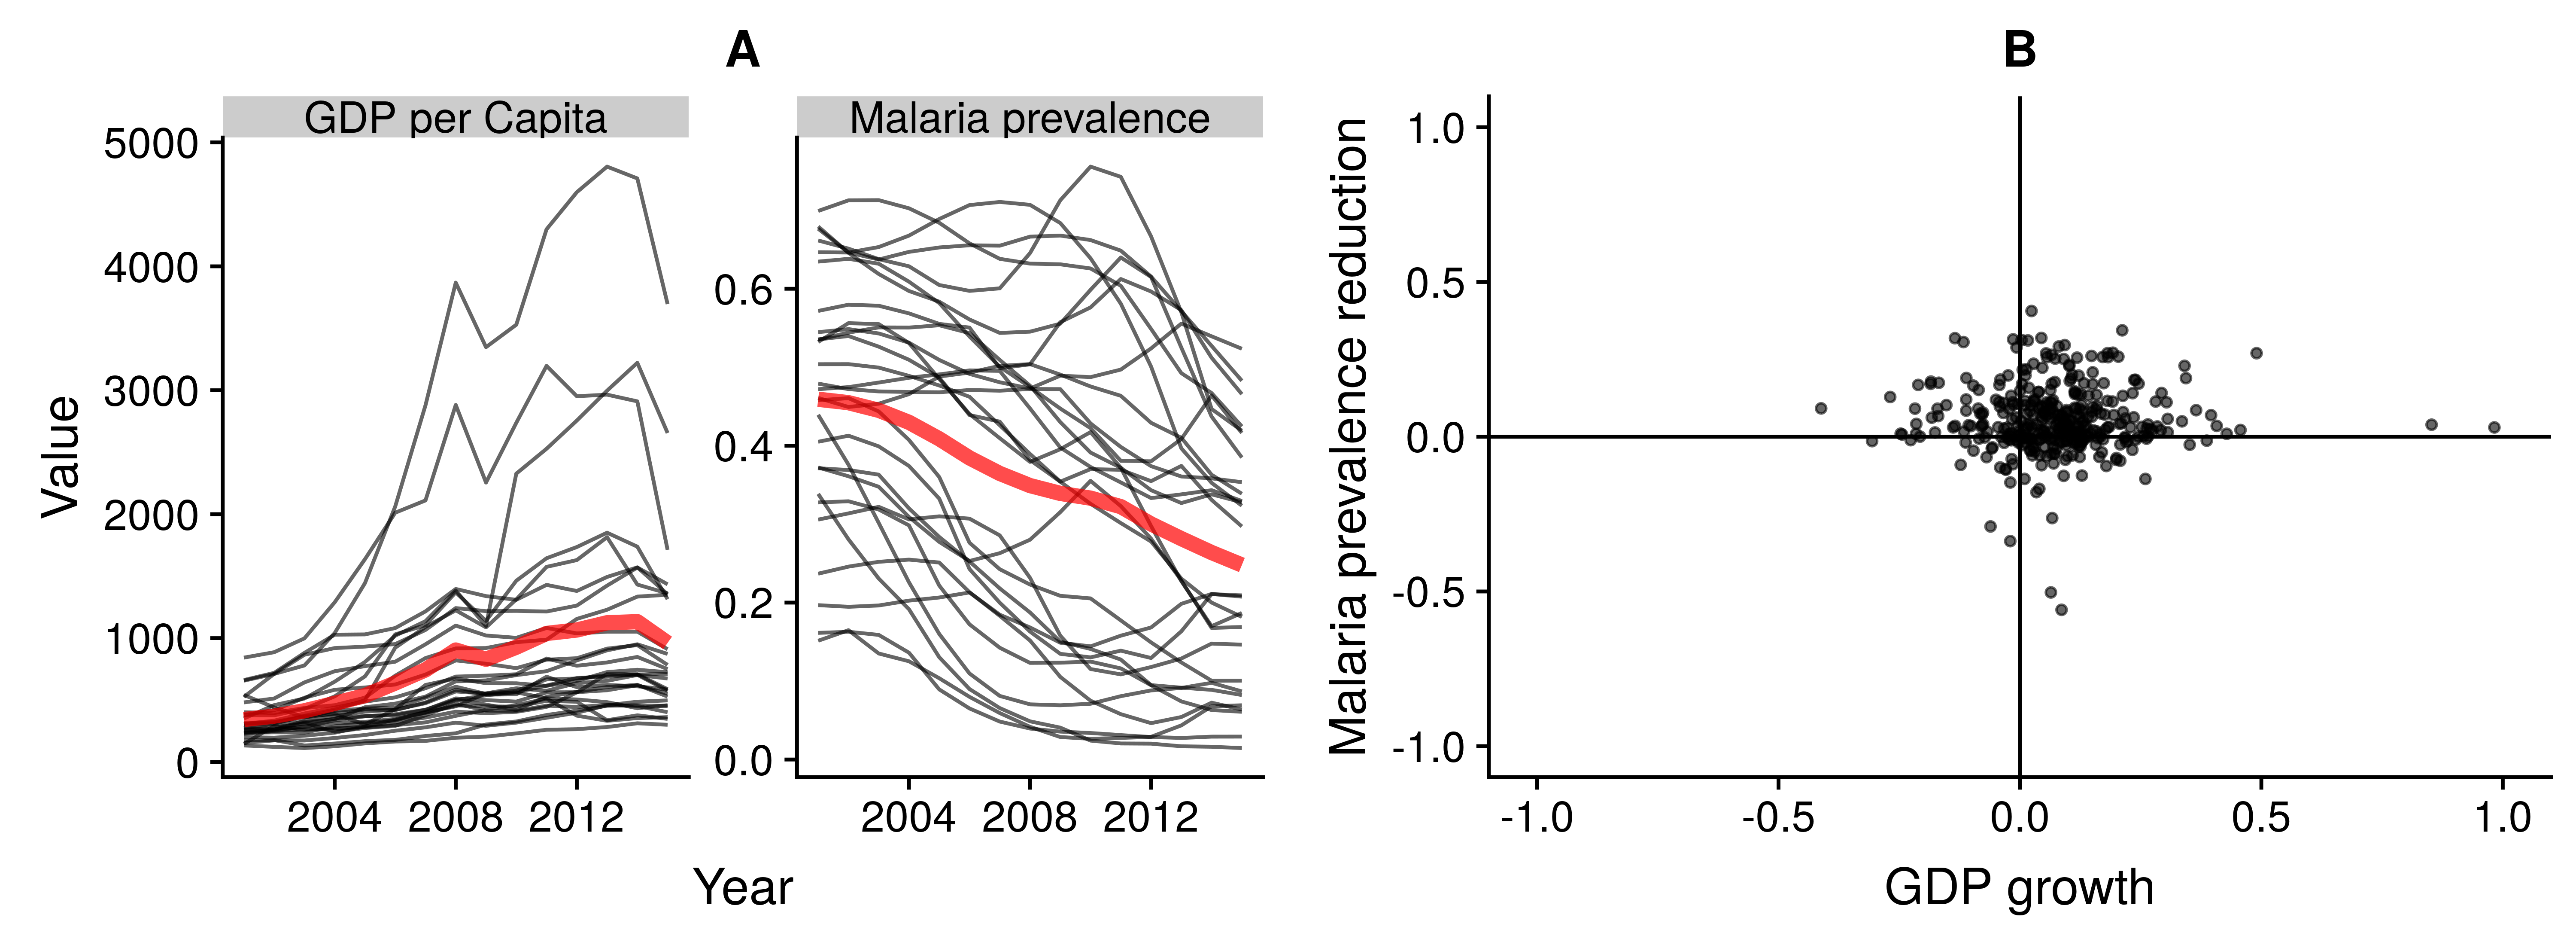
\includegraphics[width=.9\linewidth]{../figures/descriptive}
\caption{A. Country-specific GDP and malaria prevalence values during observation period (all-country average in red). B. Association of growth (GDP divided by previous year's GDP) and reduction in malaria prevalence (1 minus prevalence divided by previous year's prevalence).}
\label{fig:descriptive}
\end{figure*}


% And here is some other figure \ref{fig:paths}

% \begin{figure}%[tbhp] Remove the asterisk to get column width only
% \centering
% 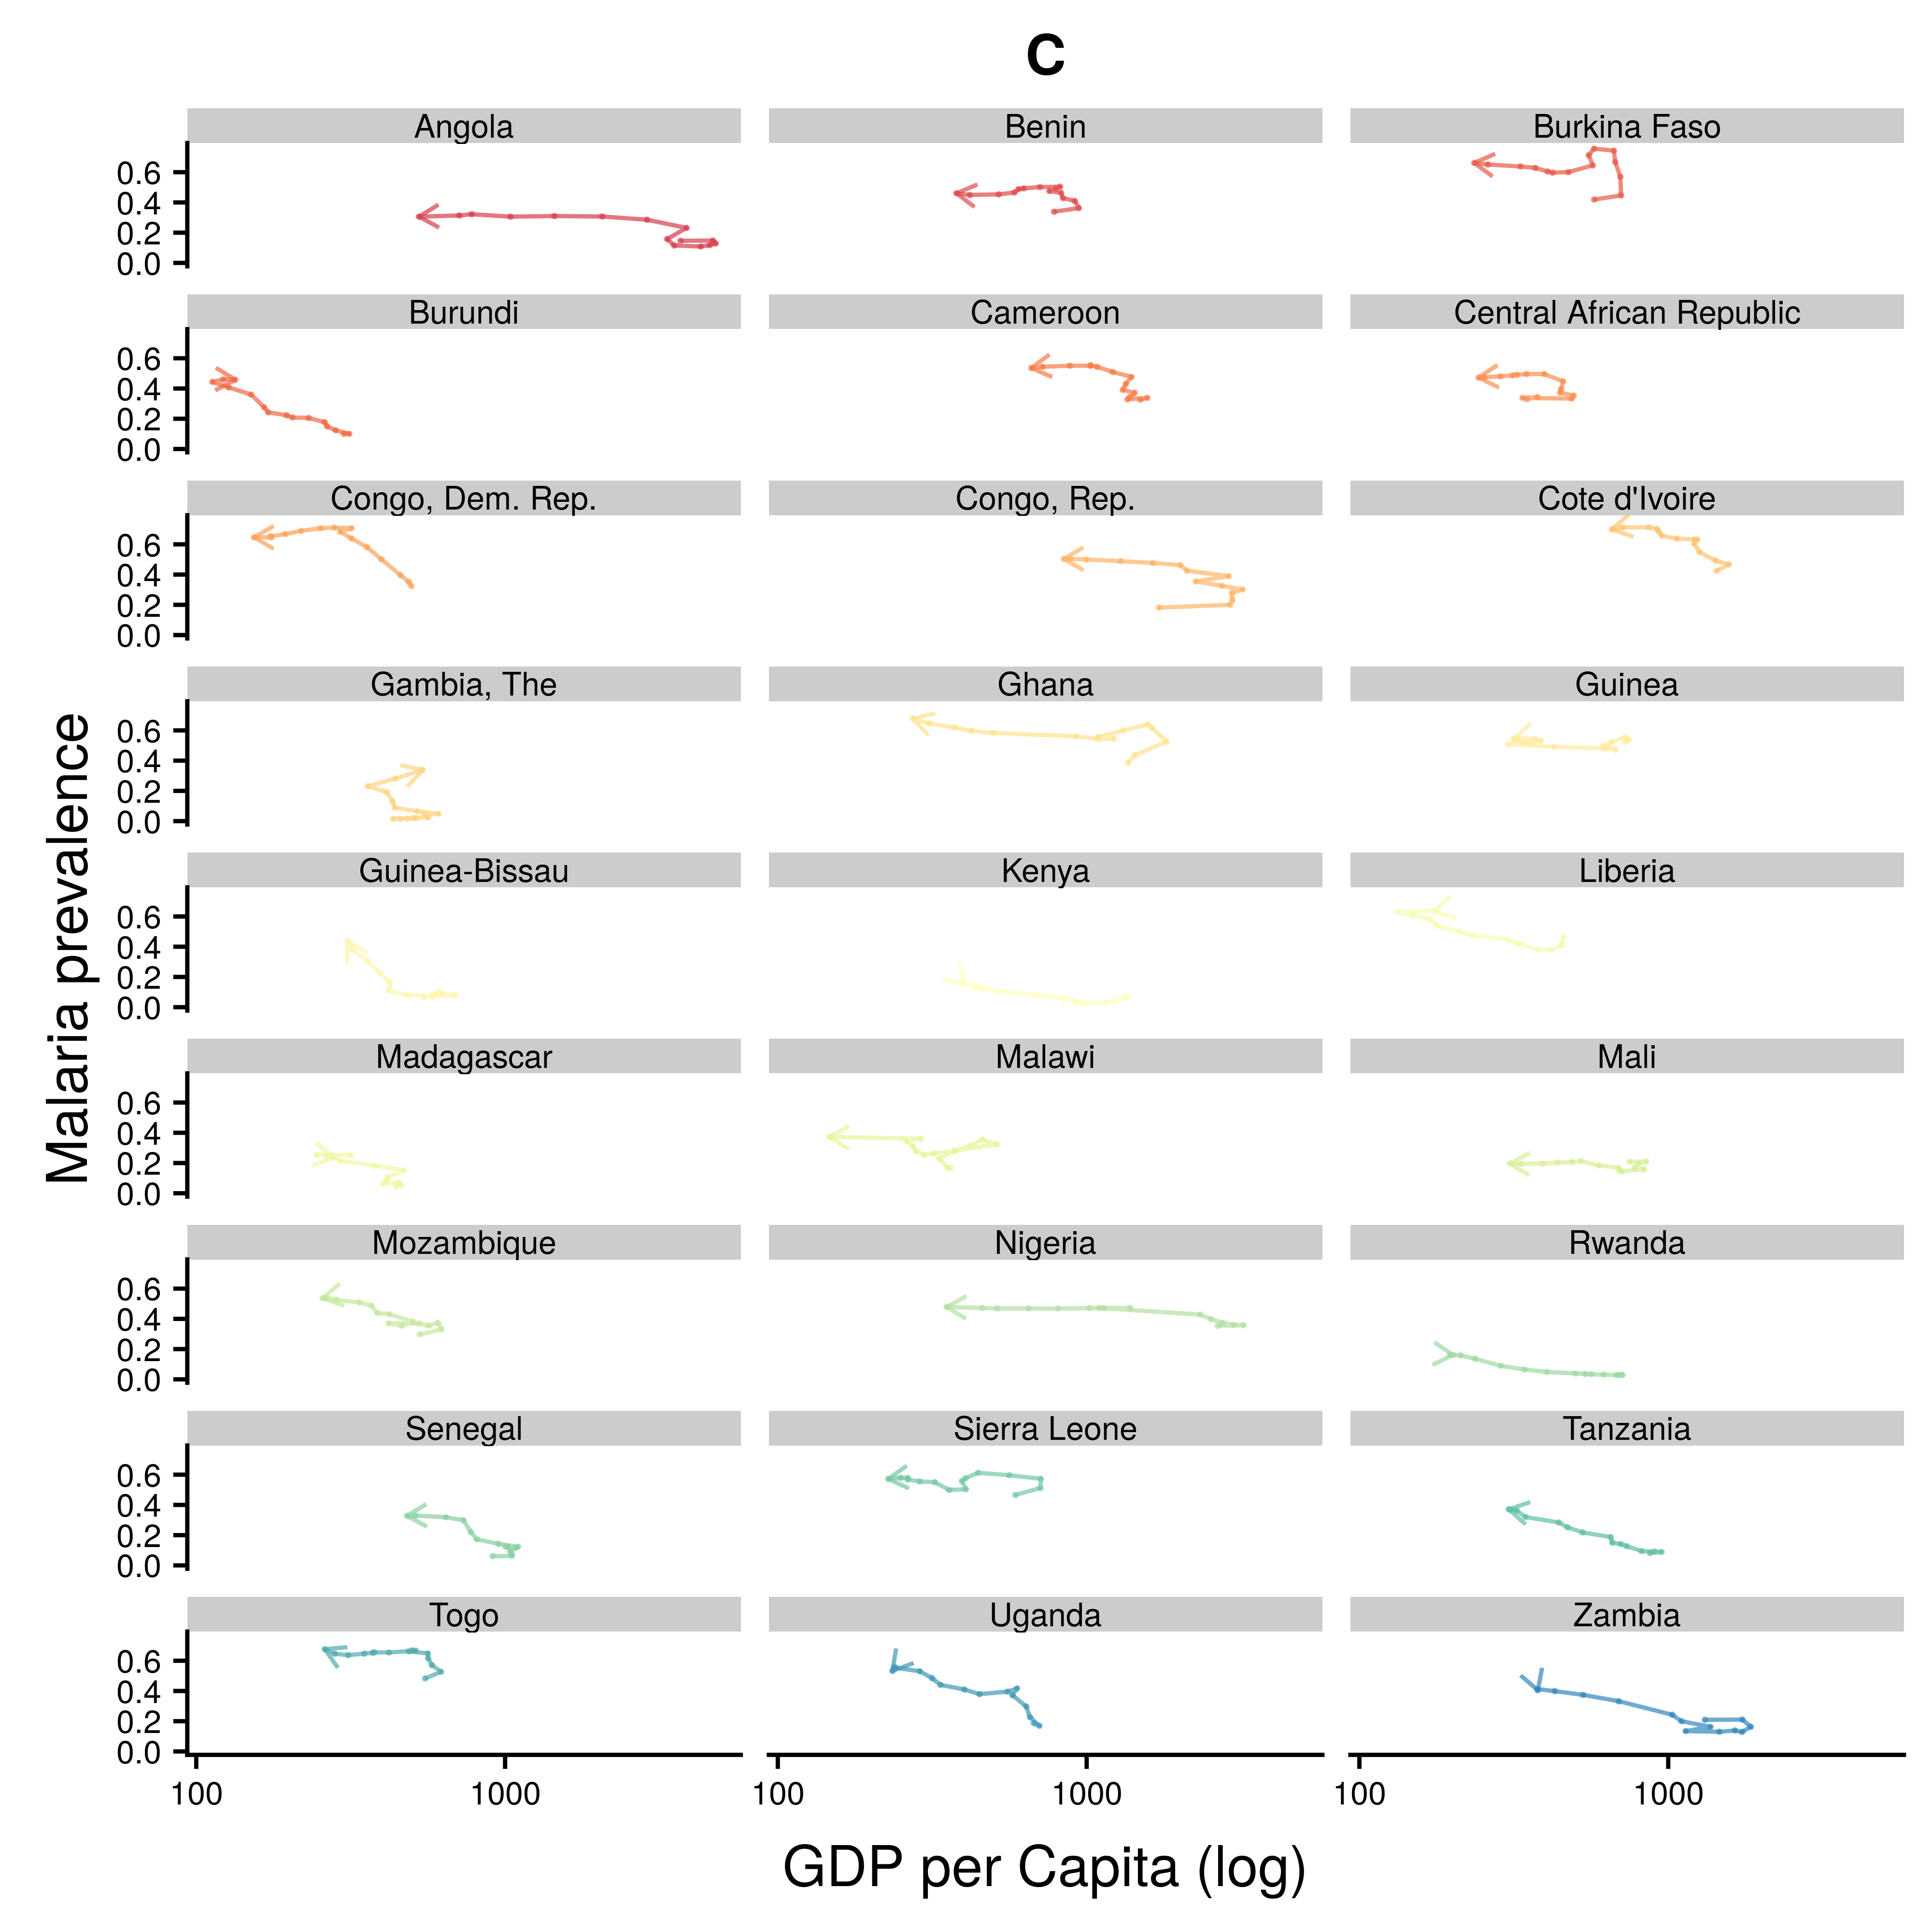
\includegraphics[width=.95\linewidth]{../figures/paths}
% \caption{GDP-Malaria trajectory, 2000-2015.}
% \label{fig:paths}
% \end{figure}



\subsection*{Granger causality}


\subsection*{Sensitivity analysis}

\section*{Discussion}

Bidirectional. Our finding that health affects wealth more than vice-versa is consistent with NOTME: Asafu-Adjaye’s (2004) study of 44 developing and developed countries and to the overall results of Erdil and Yetkiner (2009) and . It’s also consistent with Clarke’s finding that health’s causal importance was greater among low-income countries (Clarke JA 2016).





\subsection*{Digital Figures}


Figures and Tables should be labelled and referenced in the standard way using the \verb|\label{}| and \verb|\ref{}| commands.

Figure \ref{fig:frog} shows an example of how to insert a column-wide figure. To insert a figure wider than one column, please use the \verb|\begin{figure*}...\end{figure*}| environment. Figures wider than one column should be sized to 11.4 cm or 17.8 cm wide. Use \verb|\begin{SCfigure*}...\end{SCfigure*}| for a wide figure with side captions.

\subsection*{Tables}
In addition to including your tables within this manuscript file, PNAS requires that each table be uploaded to the submission separately as a “Table” file.  Please ensure that each table .tex file contains a preamble, the \verb|\begin{document}| command, and the \verb|\end{document}| command. This is necessary so that the submission system can convert each file to PDF.

\subsection*{Single column equations}

Authors may use 1- or 2-column equations in their article, according to their preference.

To allow an equation to span both columns, use the \verb|\begin{figure*}...\end{figure*}| environment mentioned above for figures.

Note that the use of the \verb|widetext| environment for equations is not recommended, and should not be used. 

\begin{figure*}[bt!]
\begin{align*}
(x+y)^3&=(x+y)(x+y)^2\\
       &=(x+y)(x^2+2xy+y^2) \numberthis \label{eqn:example} \\
       &=x^3+3x^2y+3xy^3+x^3. 
\end{align*}
\end{figure*}


\begin{table}%[tbhp]
\centering
\caption{Comparison of the fitted potential energy surfaces and ab initio benchmark electronic energy calculations}
\begin{tabular}{lrrr}
Species & CBS & CV & G3 \\
\midrule
1. Acetaldehyde & 0.0 & 0.0 & 0.0 \\
2. Vinyl alcohol & 9.1 & 9.6 & 13.5 \\
3. Hydroxyethylidene & 50.8 & 51.2 & 54.0\\
\bottomrule
\end{tabular}

\addtabletext{nomenclature for the TSs refers to the numbered species in the table.}
\end{table}

\matmethods{Data on the estimated Plasmodium falciparum parasite rate in 2-10 year olds from the period from 2000 through 2015 was obtained from the Malaria Atlas Project \cite{Hay_2006, Guerra_2007}. Annual Gross Domestic Product (GDP) per capita data was obtained from the World Bank \cite{worldbank}. We used the raster package \cite{raster} to aggregate point-specific Pf rates into annual country-wide averages (henceforth referred to as "Malaria prevalence"). All data processing and analysis was carried out in R \cite{rr}, and all data and code are freely available online \cite{brew}. Following the construction of our panel dataset, we used the PML package for the estimation of our Granger causality models \cite{Croissant_2008}.}

\showmatmethods % Display the Materials and Methods section

\pnasbreak


% Bibliography
\bibliography{pnas-sample}

\end{document}